\newcommand{\assignmentDate}{November 18th, 2019}

% Add title
%Institute
\begin{tabular*}{\hsize}{l@{\extracolsep{\fill}} r}
	\textsc{Technical University of Berlin}		 \hfill&								 	\\
	Faculty II - Mathematics and Natural Sciences\hfill&									\\
	Institute of Mathematics 					 \hfill&									\\
	Dr. D. Peschka, A. Selahi 		 			 \hfill&									\\
\end{tabular*}

% Title
\begin{center}
	\textbf{\Large{\courseName}}\\
	\vspace{7pt}
	\large{Homework \currentAssignment}\\
	\smallskip
	\normalsize{Submitted on \assignmentDate}
\end{center}

% Group table
\begin{center}
	\vspace{-8pt}
	\begin{tabular}{l c r}
		by \textbf{\groupNumber}		    &	 			  &		 								\\
		\hline
		\texttt{Kagan Atci} 			    & \texttt{338131} & \texttt{Physical Engineering, M.Sc.}\\
		\texttt{Navneet Singh }		 	    & \texttt{380443} & \texttt{Scientific Computing, M.Sc.}\\ 
		\texttt{Daniel V. Herrmannsdoerfer} & \texttt{412543} & \texttt{Scientific Computing, M.Sc.}\\ 
		\hline
	\end{tabular}
\end{center}

% EXERCISE 1
% --------------------------------------------------------------------------------------------------------------------
\addExercise{1}{Ex1}
Considered is the Laplace operator $Lu = -\Delta$ in $\Omega = (0, L)^2$ and $u \in C^4(\bar{\Omega})$.
%
% ----------------
\newcommand{\bigO}[1]{\mathcal{O}(#1)}
\newcommand{\fixDot}{\;\cdot\;}
\addSubExercise{a}
Let $\VECT{x} = [x_1, x_2]^T \in \Omega_h$.
Applying the Laplace operator in the form of finite difference on $u(\VECT{x})$ takes place by differentiating $u(\VECT{x})$ with respect to $x_1$ and $x_2$ one at a time.
The $D^-D^+$ stencil is employed as the 2nd order finite difference operator with one neighbor on either side at the distance $h$.
\begin{align}
	\label{eq:diffX1}
	\frac{\partial^2u}{\partial x_1 ^2} = D^-D^+u(x_1 ,\fixDot) = \frac{u(x_1 + h, x_2) - 2u(x_1, x_2) + u(x_1 - h, x_2)}{h^2} + \bigO{h^2}\\
	\label{eq:diffX2}
	\frac{\partial^2u}{\partial x_2 ^2} = D^-D^+u(\fixDot, x_2) = \frac{u(x_1, x_2 + h) - 2u(x_1, x_2) + u(x_1, x_2 - h)}{h^2} + \bigO{h^2}
\end{align}
With remainders neglected in Equations (\ref{eq:diffX1}) and (\ref{eq:diffX2}), the Laplace operator can be approximated by adding both equations
\begin{equation}
	\label{eq:deltaU}
	\Delta u \approx \frac{u(x_1 + h, x_2) + u(x_1, x_2 + h) - 4u(x_1, x_2) + u(x_1 - h, x_2) + u(x_1, x_2 - h)}{h^2} \text{.}
 \end{equation}
Since $u$ is a four times continuously differentiable function in $\bar{\Omega}$ and the remainder is $\bigO{h^2}$, it holds $|| f_h -L_h R_h u||_{h} \in \bigO{h^2}$ as $h\rightarrow 0$, where $f_h$ is the right hand side of the BVP, $L_h$ the finite difference matrix and $R_h$ the restriction operator within $\bar{\Omega}$.
Hence, \EQ{deltaU}, also called as the 5-point stencil, is considered as a 2nd order consistent approximation of $\Delta u$.
%
% ----------------
\addSubExercise{b}

%
% ----------------
\addSubExercise{c}

%
% ----------------
\addSubExercise{d}
\begin{figure}[H]
	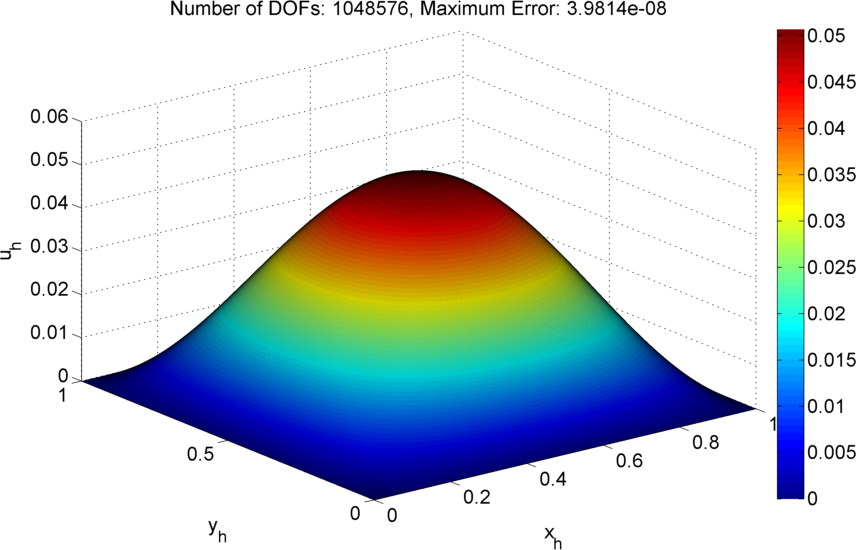
\includegraphics[width=\textwidth]{a04ex01Laplace.png} 
	%\caption{Maximum error $\max_i|u_h (ih)-u(ih)|$ between the approximation and the exact solution}
	\label{fig:a04ex01Laplace}
\end{figure}

%
% EXERCISE 2
% --------------------------------------------------------------------------------------------------------------------
\addExercise{2}{Ex2}
%
% ----------------
\addSubExercise{a}

%
% ----------------
\addSubExercise{b}

%
% EXERCISE 3
% --------------------------------------------------------------------------------------------------------------------
\addExercise{3}{Ex3}
%
% ----------------
\addSubExercise{a}

%
% ----------------
\addSubExercise{b}

%
% ----------------
\addSubExercise{c}

%
% ----------------
\addSubExercise{d}